\documentclass[12pt] {article}
\usepackage{times}
\usepackage[margin=1in,bottom=1in,top=1in]{geometry}

\usepackage{hhline}
\usepackage{subfig}
\usepackage{amsmath}
\usepackage{amsfonts}
\usepackage[inline,shortlabels]{enumitem}%enumerate with letters
\usepackage{mathrsfs} 
\usepackage[square,numbers]{natbib}
\usepackage{graphicx}
\bibliographystyle{unsrtnat}
\begin{document}

\title{Assignment Five -  EEC254}
\author{Ahmed H. Mahmoud}
\date{February 20th, 2018}
\maketitle

%============Table========
%\begin{figure}[tbh]
% \centering    
%\begin{tabular}{ |p{4cm}|| p{2cm}|p{2cm}|p{2cm}|p{2cm}|}
% \hline
% & Processor 1 &  Processor 2  & Processor 3 & Processor 4\\ \hhline{|=|=|=|=|=|}
% \hline
% Performance          &$1.08$        &$1.425$       &\textbf{1.52}  &   \\
% \hline
%\end{tabular} 
%\caption{Metric table for the four processors}
%   \label{tab:metric}
%\end{figure} 
%============Figure========
%\begin{figure}[!tbh]
%\centering        
%   \subfloat {\includegraphics[width=0.65\textwidth]{fig2_4.png}}
%   \caption{ }
%   \label{fig:fig}
%\end{figure}

%\begin{enumerate}[(a)]
%\end{enumerate}


\paragraph{Problem 5.1:} 
\begin{enumerate}[(a)]
\item $2\leq x \leq 4$ is the feasible set. $p^{*}=5$ is the optimal value.  $x^{*}=2$ is the optimal solution. 
\item The Lagrangian for this problem is $L(x,\lambda)=f_{0}(x) + \lambda f_{1}(x) = (x^{2}+1) + 
\lambda \left(x^{2}-6x+8 \right)$. Figure~\ref{fig:5_1_b}(a) shows the objective function, constraints and the Lagrangian for different $\lambda$ values. The minimum value of the Lagrangian increases from $0 \leq \lambda \leq 2 $ and then decreases for greater vales of $\lambda$. At $\lambda =2$, the minimum value is the maximum we can obtain i.e., 5. This verifies the \textbf{lower bound property}.

\begin{figure}[!tbh]
\centering        
   \subfloat [Lagrangian] {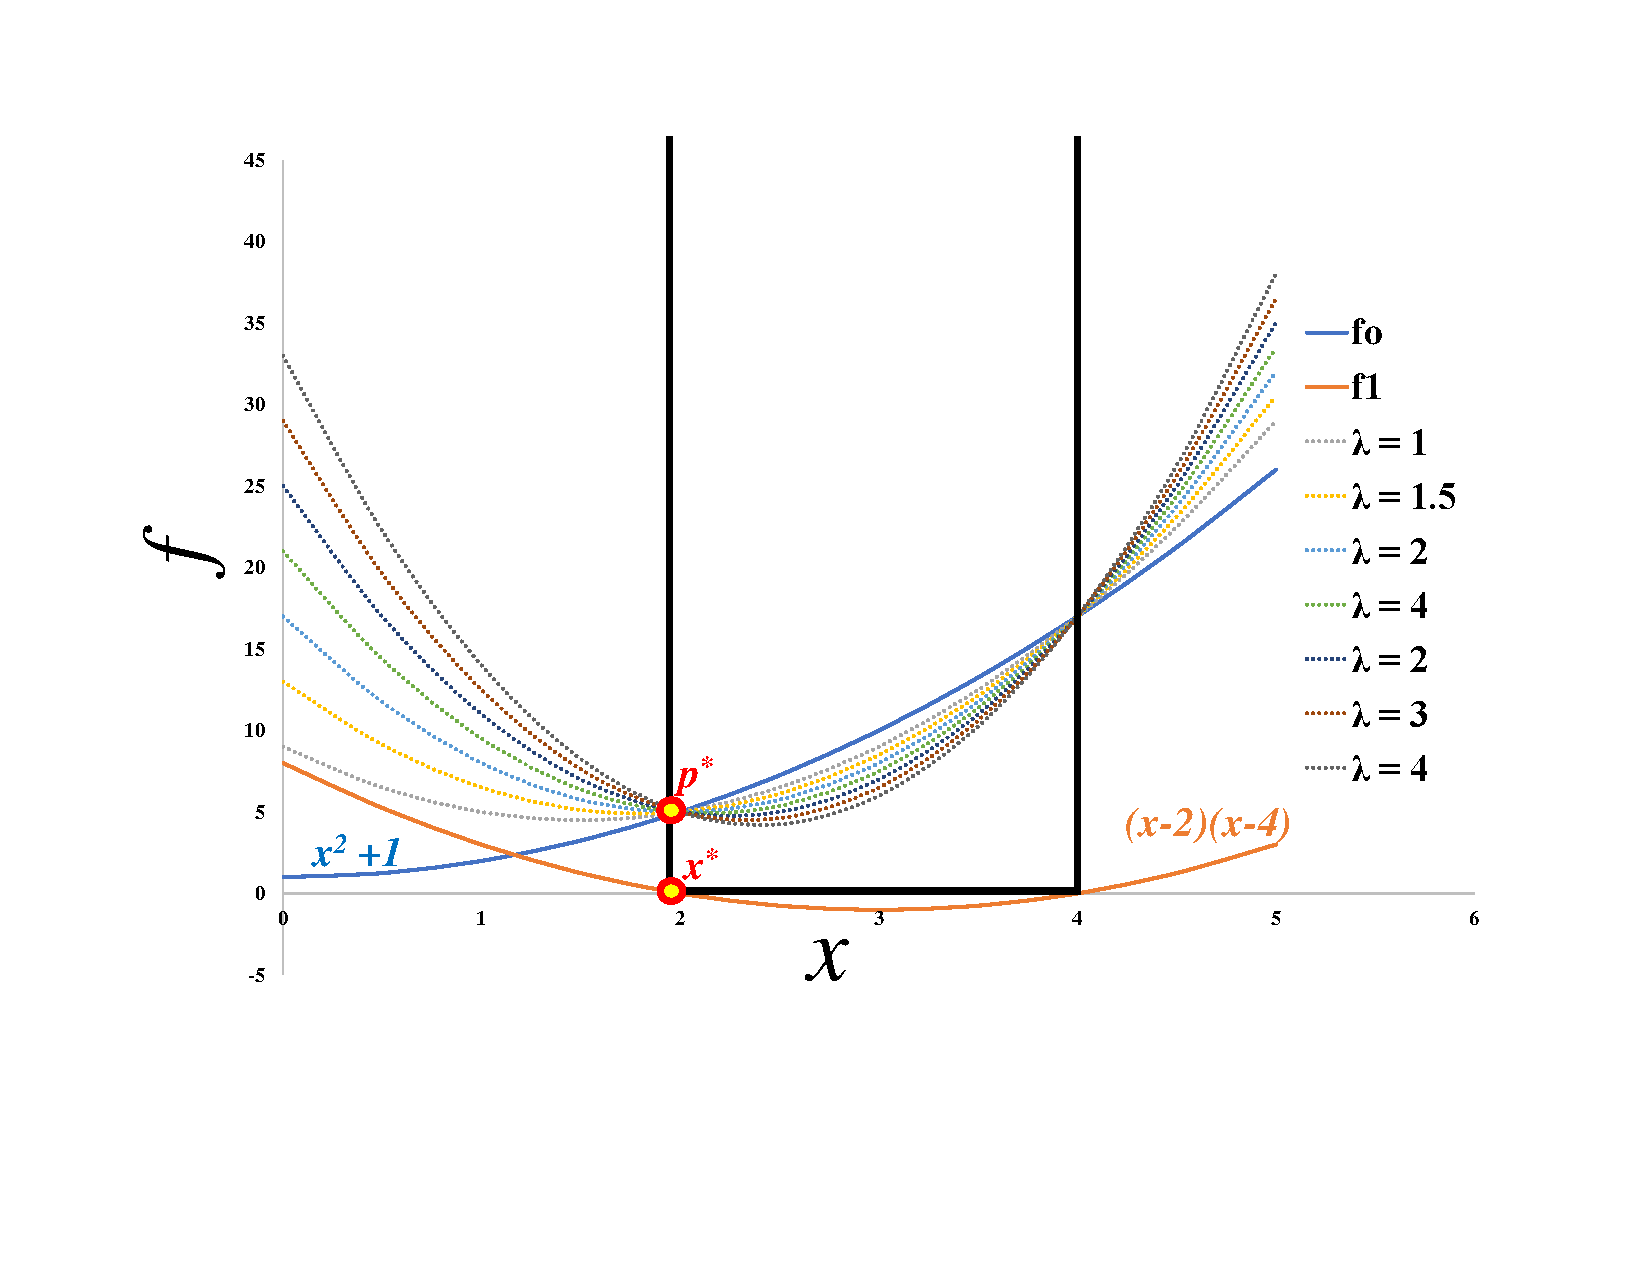
\includegraphics[width=0.49\textwidth]{5_1b1.pdf}}
   \subfloat [Dual function] {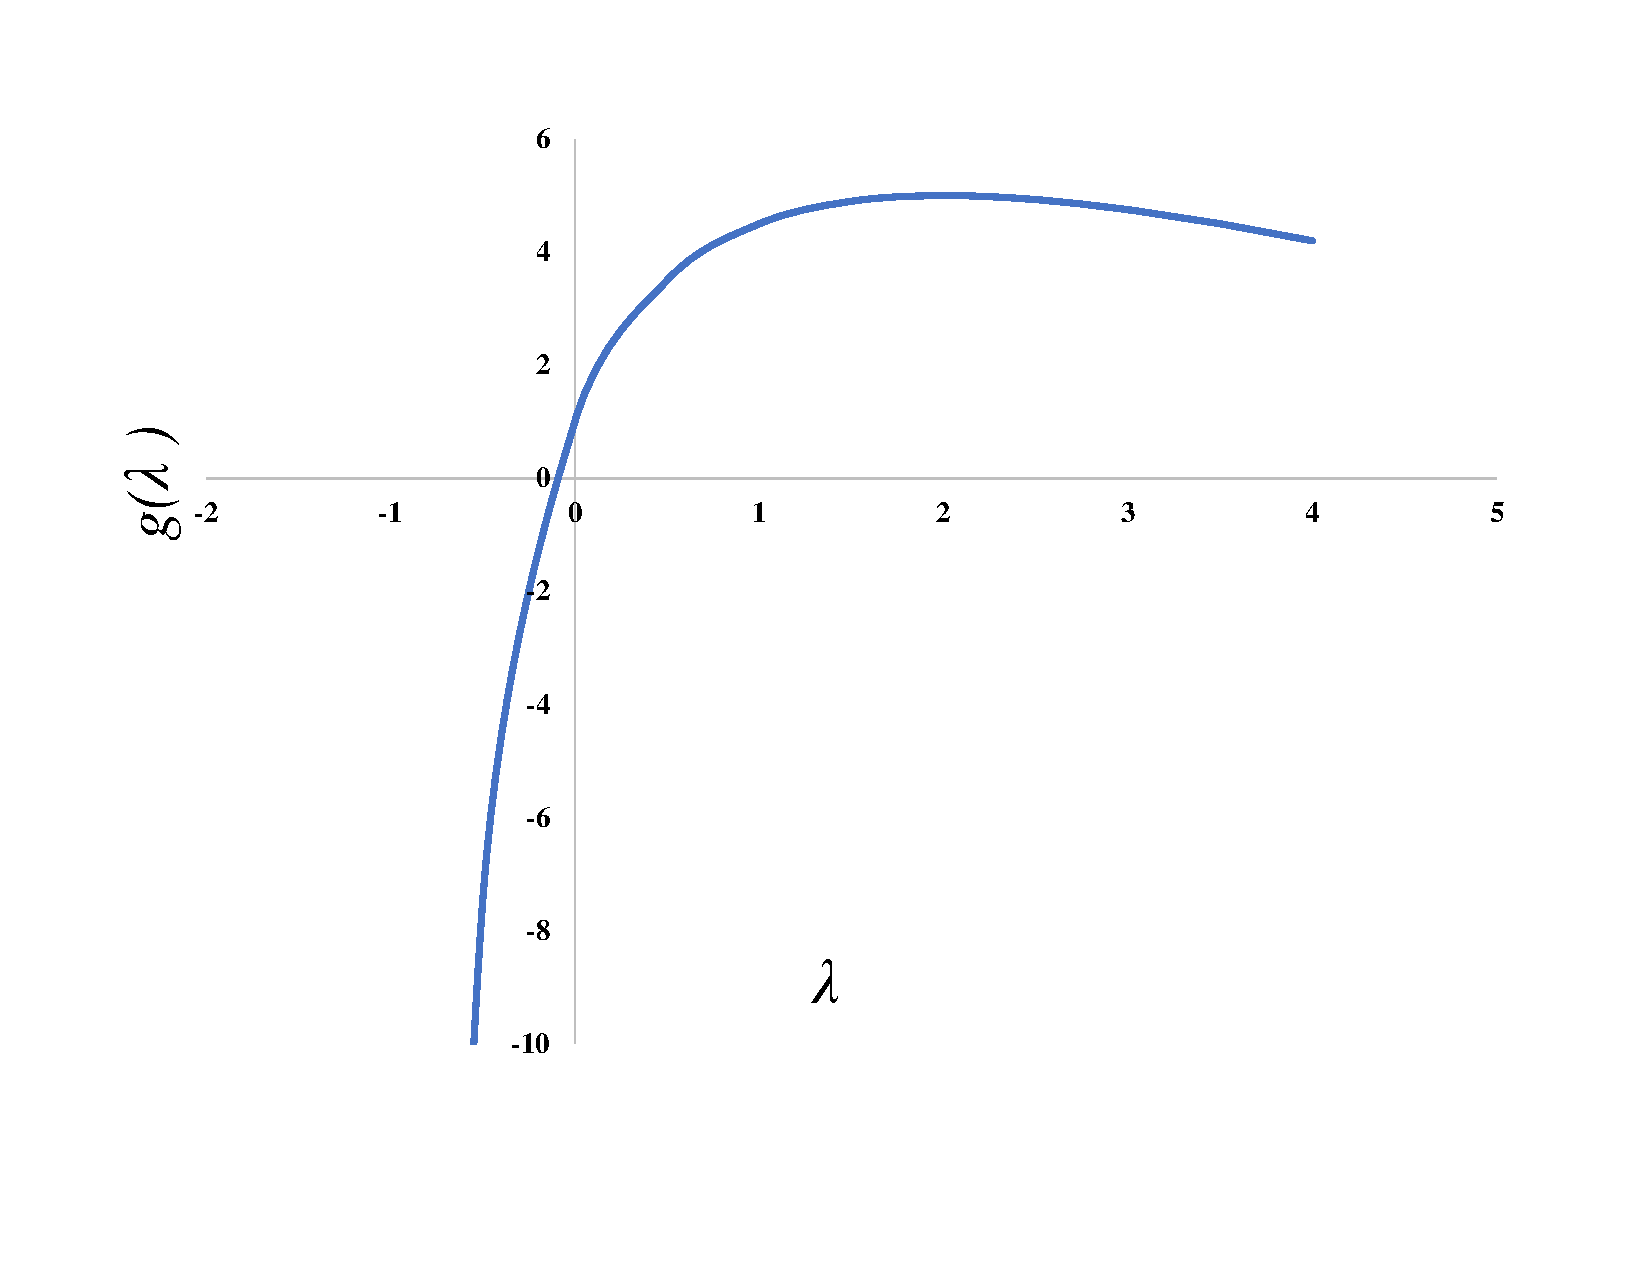
\includegraphics[width=0.49\textwidth]{5_1b2.pdf}}
   \caption{(a) Plot of $f_{0}(x) = x^{2}+1$, $f_{1}(x) =(x-2)(x-4)$ and the Lagrangian for different $\lambda$. The feasible region is inside the black box. The optimal solution $x^{*}=2$ and the optimal value $p^{*}=5$. (b) the dual function $g(\lambda)$.}
   \label{fig:5_1_b}
\end{figure}

The dual function is defined as $g(\lambda) = inf_{x} (1+\lambda)x^{2} - 6\lambda x + (1+8\lambda)$. We notice that when $x^{2}$ coefficient is non-positive, the problem becomes unbounded below. Thus, for $\lambda \leq -1$, the problem is unbounded below. Other wise, the minimum value of this quadratic function occurs at $x = \frac{-(-6\lambda)}{2(1+\lambda)} = \frac{3\lambda}{1+\lambda}$. Thus the dual function can be written as 
$$
g(\lambda)=
\begin{cases}
   \frac{-9\lambda^{2}}{1+\lambda}+1+8\lambda \quad \lambda > -1 \\    
   -\infty            \quad \quad \quad \quad \quad \lambda \leq -1 \\    
\end{cases}
$$
Figure ~\ref{fig:5_1_b}(b) shows the plot of the dual function. 
\item The dual problem can be written as 
\[
\begin{array}{cl}
\text{maximize} & \frac{-9\lambda^{2}}{1+\lambda}+1+8\lambda\\
\text{subject to} & \lambda \geq 0
\end{array} 
\]
Form (b), the dual optimal value is 5 at $\lambda^{*} =2$. Thus, strong duality exists. From the plot of $g(\lambda)$ (Figure~\ref{fig:5_1_b}(b)) we can verify that the problem is concave maximization since $g(\lambda)$ is concave function. 

\item Since the minimum value $x^{2}-6x +8$ can take is -1, then the perturbed problem is infeasible if $u<-1$. When $u=-1$, there is one feasible point; the intersection of the vertical line $x=3$ and the objective function. As $u$ increases, the feasible set (window) is widened upto $u\geq 8$ at which point the problem becomes unconstrained and the optimum value become $1$ at $x^{*}=0$. Before that, the optimum value occurs at the smaller root of the constraints inequality $(x-2)(x-4)\leq u$ since $x^{2}+1$ is monotonically increasing. The smaller root of $(x-2)(x-4)=u$  is $x=-\sqrt{u +1}+3$. Thus the optimum value for the perturbed problem as a function of $u$ is 

$$
p(u)=
\begin{cases}
	\infty \qquad \qquad \qquad \qquad \qquad u< -1 \\
	11 + u - 6\sqrt{1+u} \qquad -1\leq u \leq 8 \\
	1 \qquad \qquad \qquad \qquad \qquad \quad u\geq 8
\end{cases}
$$
Figure~\ref{fig:5_1_d} shows $p^{*}(u)$ as a function of $u$. Taking the derivative of $p^{*}(u)$, we get $\frac{dp^{*}(u)}{du} = 1 - \frac{3}{\sqrt{1+u}}$. At $u=0$, we have $\frac{dp^{*}(0)}{du} = -2 = -\lambda^{*}$.

\begin{figure}[!tbh]
\centering        
   \subfloat {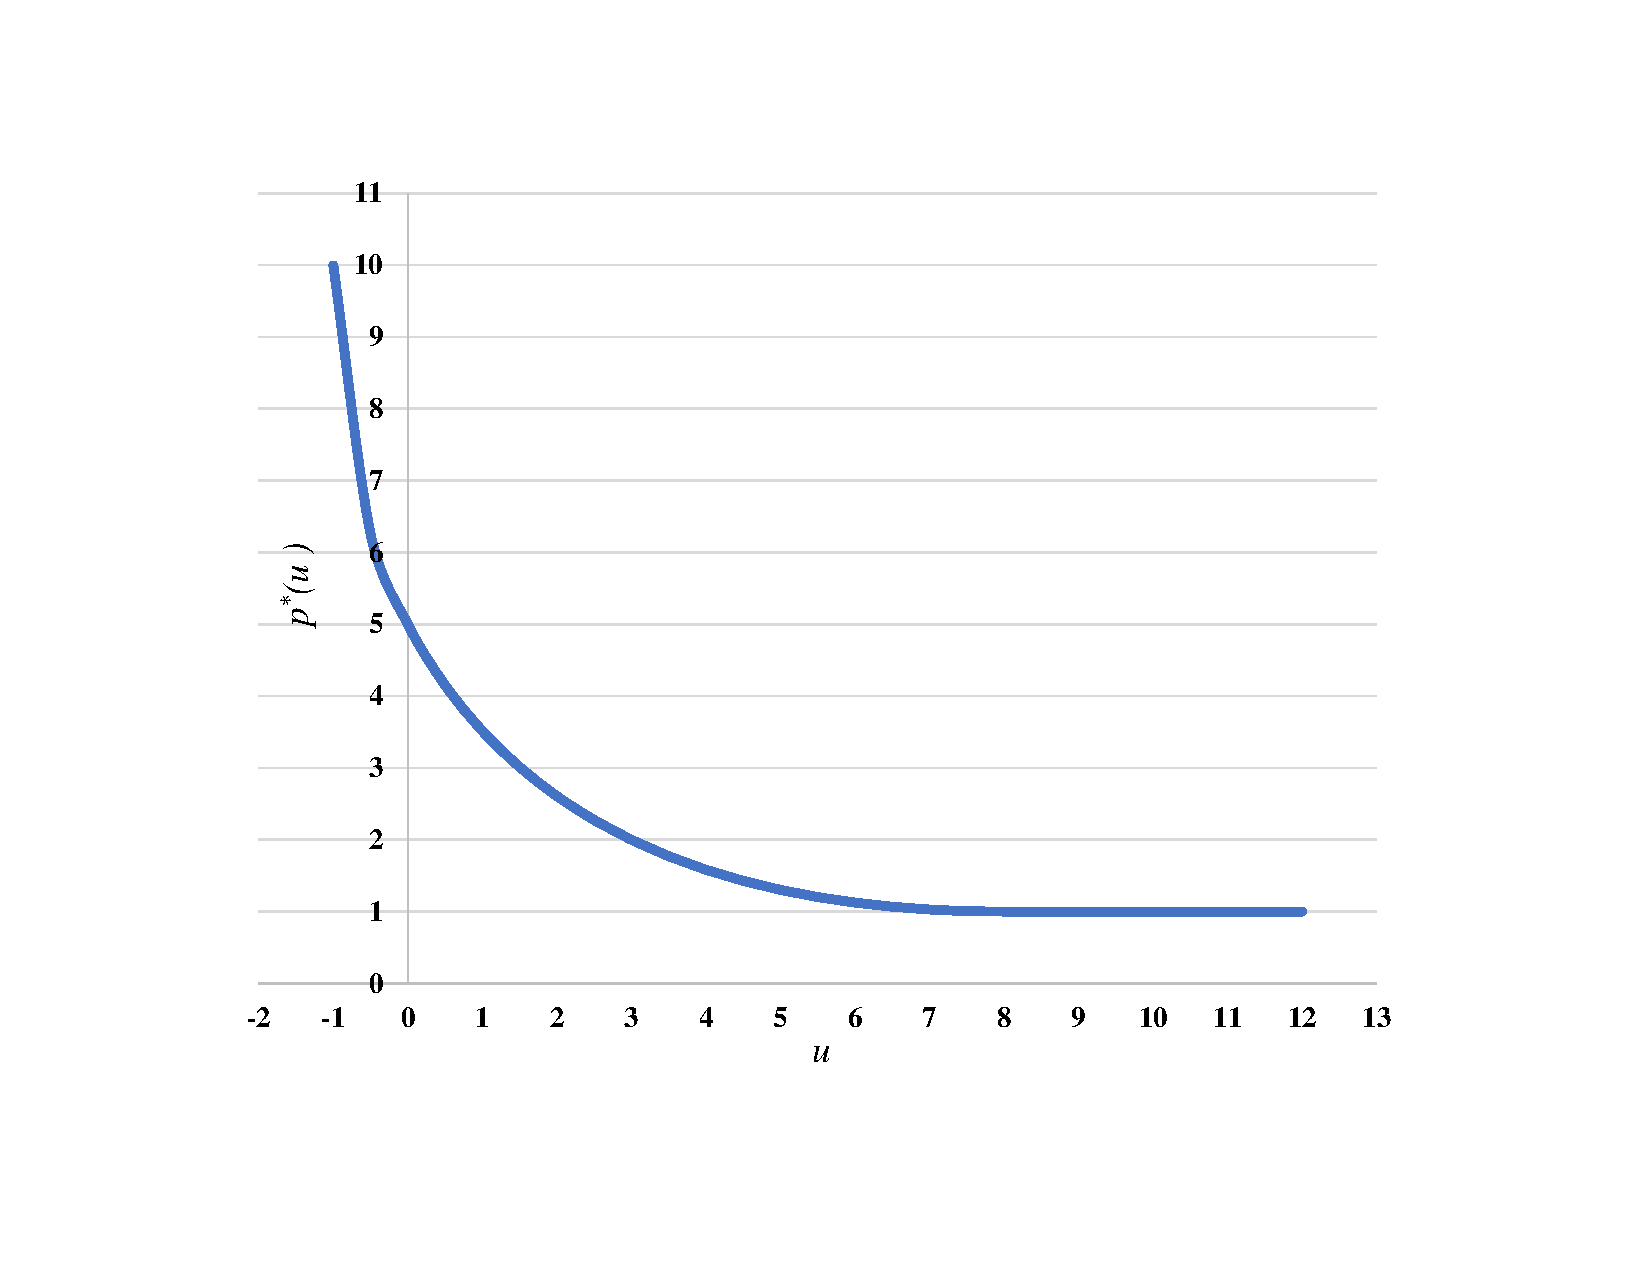
\includegraphics[width=0.49\textwidth]{5_1d.pdf}}
   \caption{The optimal value of the perturbed version of the problem in Problem 5.1 as a function of $u$}
   \label{fig:5_1_d}
\end{figure}

\end{enumerate}

\paragraph{Problem 5.20:} 
The Lagrangian of this problem can be expressed as 
$$
L(x,y,\lambda, \nu) = -c^{T}x + \sum^{m}_{i=1}y_{i}\ log\ y_{i} - \lambda^{T}x + \nu_{0}(\textbf{1}^{T}x -1) + \nu_{1}^{T}(Px-y)
$$
$\lambda$ takes a negative sign since we have to flip $x$'s inequality. The objective function is in two variables, $x$ and $y$, and so the Lagrangian has to be as a function of them (along with Lagrange multiplier vectors; $\lambda$,$\nu$).  

$$
L(x,y,\lambda, \nu) = (P^{T}\nu_{1} + \nu_{0}\textbf{1} -\lambda -c)^{T} x + \sum^{m}_{i=1}y_{i}\ log\ y_{i} - \nu_{0} - \nu^{T}_{1}y
$$
In order to realize the dual function, we take the infimum of the Lagrangian over $x$ followed by the infimum of it over $y$. Since $(P^{T}\nu_{1} + \nu_{0}\textbf{1} -\lambda -c)$ is a linear function, then the infimum of the dual function over $x$ is bounded below only if $(P^{T}\nu_{1} + \nu_{0}\textbf{1} -\lambda -c) = 0$. Thus
\[
inf_{x}L(x,y,\lambda, \nu) = \sum^{m}_{i=1}y_{i}\ log\ y_{i} - \nu_{0} - \nu^{T}_{1}y
\]

To take the infimum of the above over $y$, we are going to use the results in Section 5.1.6 about the Entropy maximization problem and the relation between the dual and conjugate function (in (5.11) and (5.13)). From that we get,
\[
inf_{y} \left( \sum^{m}_{i=1}y_{i}\ log\ y_{i} - \nu_{0} - \nu^{T}_{1}y \right) = -\nu_{0} -\sum_{i=1}^{m}e^{\nu_{1}-1} 
\]
Finally, the dual problem is
\[
\begin{array}{cl}
\text{maximize} & -\nu_{0} -\sum_{i=1}^{m}e^{\nu_{1}-1} \\
\text{subject to} & (P^{T}\nu_{1} + \nu_{0}\textbf{1} -\lambda -c) \succeq 0
\end{array} 
\]

\paragraph{Problem 5.26:} 
\begin{enumerate}[(a)]
\item The objective function level sets is circles centered at the origin. The feasible region is the intersection of 1) unit circle centered at $(1,1)$ 2) unit circle centered at $(1,-1)$. Thus, the feasible set is just one point at $(1,0)$ and it is the optimal point $x^{*}$ with optimal value  $p^{*}=1$. Figure ~\ref{fig:5_26_a} shows the level sets, feasible set and optimal point. 

\begin{figure}[!tbh]
\centering        
   \subfloat [Lagrangian] {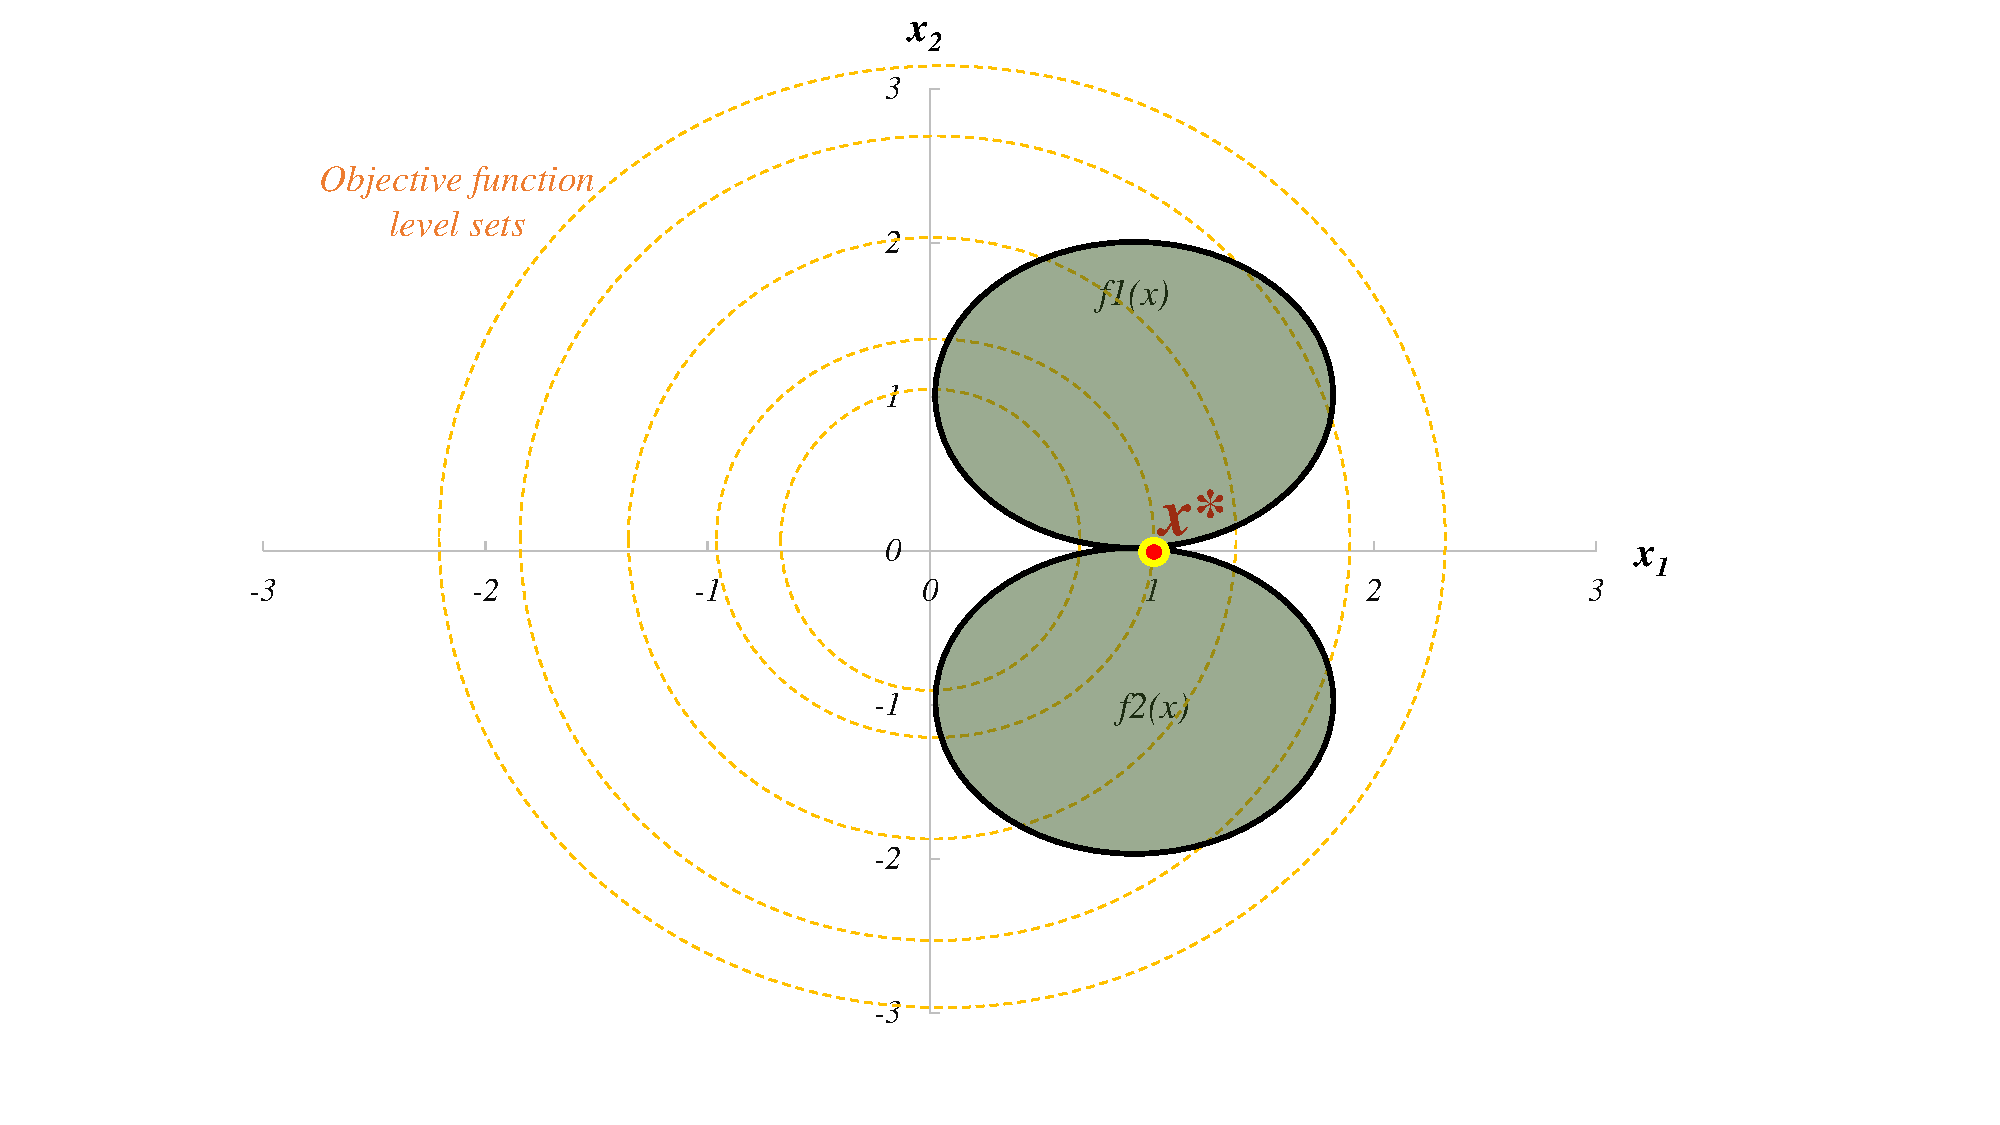
\includegraphics[width=0.49\textwidth]{5_26a.pdf}}
   \caption{Objective function level sets (dotted), feasible regions (one point) and the optimal point $x^{*}$ for Problem 5.26. }
   \label{fig:5_26_a}
\end{figure}

\item The KKT conditions for this problem are
\[
\begin{array}{c}
(x_{1}-1)^{2}+(x_{2}-1)^{2}-1 \leq 0\\
(x_{1}-1)^{2}+(x_{2}+1)^{2}-1 \leq 0\\
\lambda_{1} \geq 0 \\
\lambda_{2} \geq 0 \\
\lambda_{1}\left((x_{1}-1)^{2}+(x_{2}-1)^{2}-1\right)= 0\\
\lambda_{2}\left((x_{1}-1)^{2}+(x_{2}+1)^{2}-1\right)= 0\\
2x_{1} + 2\lambda_{1}(x_{1}-1)+ 2\lambda_{2}(x_{1}-1) = 0\\
2x_{2} + 2\lambda_{1}(x_{2}-1)+ 2\lambda_{2}(x_{2}+1) = 0\\
\end{array} 
\]
Since we know the optimal point $x^{*}$, we can substitute it in the KKT to figure out if there exists Lagrange multipliers at the optimal point. Only the last KKT condition will give us some useful information such that $-2\lambda_{1}+2\lambda_{2}=0$. Given the third and forth KKT conditions, it is clear that there exists no Lagrange multipliers $\lambda^{*}_{1}$ and $\lambda^{*}_{2}$ that prove that $x^{*}$ is optimal. 

\item 
The Lagrange of this problem is 
$$
L(x_{1},x_{2}, \lambda) = x_{1}^{2} + x_{2}^{2} + \lambda_{1}\left((x_{1}-1)^{2}+ (x_{2}-1)^{2}-1\right) + \lambda_{2}\left((x_{1}-1)^{2}+ (x_{2}+1)^{2}-1\right)
$$
$$
L(x_{1},x_{2}, \lambda) = (1+\lambda_{1}+\lambda_{2})x_{1}^{2} +  (1+\lambda_{1}+\lambda_{2})x_{2}^{2} -2(\lambda_{1}+\lambda_{2})x_{1} -2 (\lambda_{1}-\lambda_{2})x_{2}+\lambda_{1}+\lambda_{2}
$$
Thus the Lagrange dual function is $g(\lambda) = inf_{x_1,x_2} L(x_{1},x_{2},\lambda)$ which can be computed by taking the derivative of $L$ over $x_{1}$ once and over $x_{2}$ once and equating each to zero. 
$$
\frac{dL}{dx_{1}} = 2(1+\lambda_{1}+\lambda_{2})x_{1} - 2(\lambda_{1}+\lambda_{2}) \quad \quad \frac{dL}{dx_{2}} = 2(1+\lambda_{1}+\lambda_{2})x_{2} - 2(\lambda_{1}-\lambda_{2})
$$
for which the minimum is realized at 
$$
x_{1} = \frac{\lambda_{1}+\lambda_{2}}{1+\lambda_{1}+\lambda_{2}} \quad \quad x_{2} = \frac{\lambda_{1}-\lambda_{2}}{1+\lambda_{1}+\lambda_{2}}
$$
By substituting with the above values of $x_{1}$ and $x_{2}$ to obtain Lagrange dual function, we get 
$$
g(\lambda) =
\begin{cases}
   \frac{-2(\lambda_{1}^{2} + \lambda_{2}^{2}) }{1+\lambda_{1}+\lambda_{2}} + \lambda_{1} + \lambda_{2} \qquad \quad \lambda_{1} \geq 0,\lambda_{2} \geq 0 \\    
   -\infty            \quad \quad \quad \qquad \quad \quad \quad \quad \quad otherwise \\    
\end{cases}
$$
Finally, the Lagrange dual problem is 
\[
\begin{array}{cl}
\text{maximize} & \frac{-2(\lambda_{1}^{2} + \lambda_{2}^{2}) }{1+\lambda_{1}+\lambda_{2}} + \lambda_{1} + \lambda_{2}\\
\text{subject to} & \lambda_{1} \geq 0, \lambda_{2} \geq 0
\end{array} 
\]
$g(\lambda)$ does not have global maximum i.e., there is no dual optimum value. For that the strong duality does not hold. 
\end{enumerate}


\bibliography{mybib}
\end{document}
